\documentclass[border=15pt, multi, tikz]{standalone}
\usepackage{import}
\usepackage{scalefnt}
\subimport{./layers/}{init}
\usetikzlibrary{positioning}
\usetikzlibrary{decorations.pathreplacing,calligraphy}

\def\ConvColor{rgb:yellow,5;red,2.5;white,5}
\def\ConvReluColor{rgb:yellow,5;red,5;white,5}
\def\PoolColor{rgb:red,1;black,0.3}
\def\DcnvColor{rgb:blue,5;green,2.5;white,5}
\def\SoftmaxColor{rgb:magenta,5;black,7}
\def\SumColor{rgb:blue,5;green,15}
\def\poolsep{0.5}

\def\orga{(2,5)}
\def\orgab{(8,5)}
\def\orgac{(5,2)}
\def\orgad{(5,8)}

\def\orgb{(0,7)}
\def\orgbb{(-6,7)}
\def\orgbc{(-3,4)}
\def\orgbd{(-3,10)}

\begin{document}

\makeatletter
\tikzset{
    dot diameter/.store in=\dot@diameter,
    dot diameter=3pt,
    dot spacing/.store in=\dot@spacing,
    dot spacing=10pt,
    dots/.style={
        line width=\dot@diameter,
        line cap=round,
        dash pattern=on 0pt off \dot@spacing
    }
}
\makeatother
\scalefont{0.7}
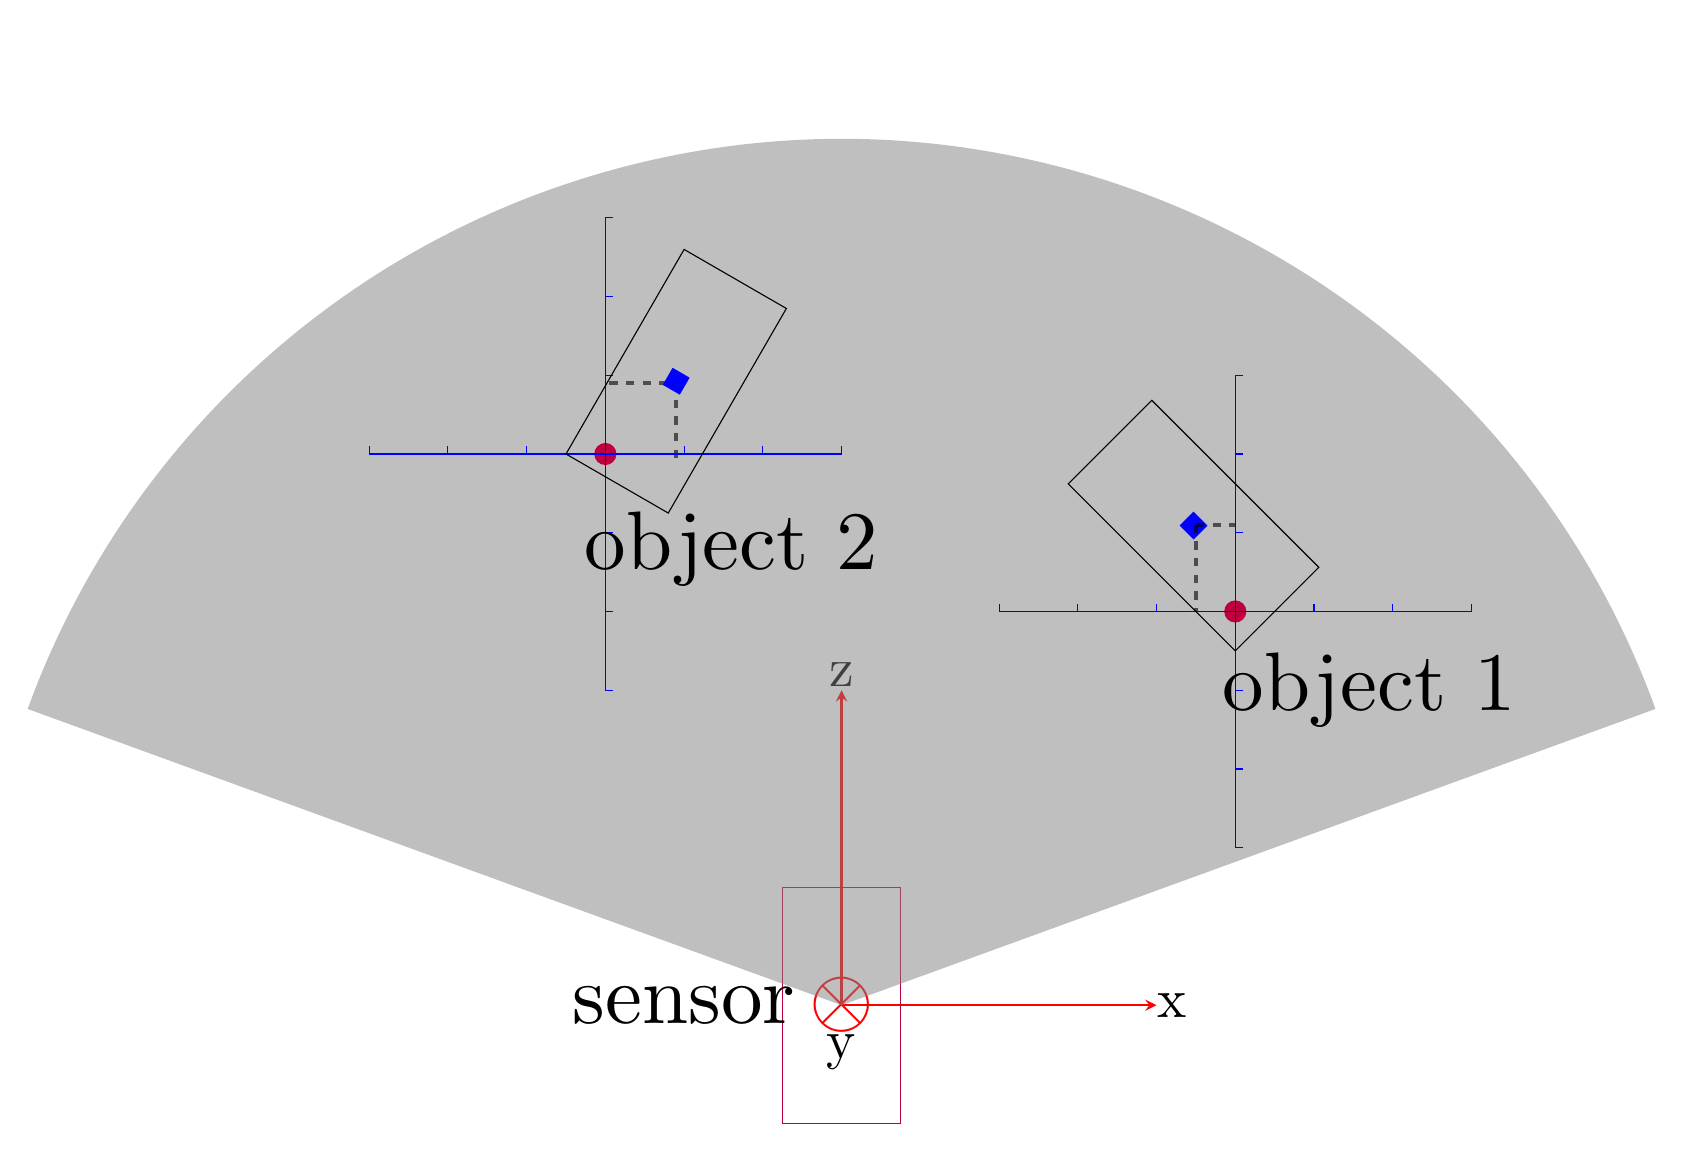
\begin{tikzpicture}
\tikzstyle{connection}=[ultra thick,every node/.style={sloped,allow upside down},draw=\edgecolor,opacity=0.6]

% sensor
\draw[-stealth, red,thick=2] (0,0)--(0,4);
\draw[-stealth, red,thick=2] (0,0)--(4,0);
\node [shift={(0,0)},align=center,scale=3,color=red] at (0,0) {$\otimes$};

\node [shift={(0,0)},align=center,scale=2] at (4.2,0) {x};
\node [shift={(0,0)},align=center,scale=2] at (0,4.2) {z};
\node [shift={(0,0)},align=center,scale=2] at (0,-0.6) {y};

% % basic coordinate
% \draw[->] (-6.5,0)--(6.5,0);
% \draw[->] (0,-0.5)--(0,12.5);

% %axis
% \foreach \x in {0,1,...,12}
% {
%     \draw[xshift=\x cm] (-6,0) -- (-6,0.1);
%     \draw[yshift=\x cm] (0,0) -- (0.1,0);
% };
% % original
% \node[below] at (0.2,0){0};
% % x scale
% \foreach \x in {-6,...,-1}
%     \node[below] at(\x,0){\x};
% \foreach \y in {1,...,6}
%     \node[below] at(\y,0){\y};
% % y scale
% \foreach \y in {1,...,12}
%     \node[left] at(0,\y){\y};
    
\draw[purple] (-0.75,-1.5) rectangle (0.75,1.5);
\fill[gray,line width=2,fill opacity=0.5] (0,0) -- (20:11) arc (20:160:11) --cycle;
\node [shift={(-2,0)}, align=center,scale=3] at (0,0) {sensor};
%%%%%%%%%%%%%%%%%%%%%%%%%%%%
%object 1
%%%%%%%%%%%%%%%%%%%%%%%%%%%%
% coor 1
\fill[purple] (5,5) circle (4pt);
\draw[-,blue] \orga --\orgab;
\draw[-,blue] \orgac --\orgad;
\foreach \x in {0,1,...,6}
{
    \draw[xshift=2cm+\x cm,yshift=5cm,blue] (0,0) -- (0,0.1);
    \draw[xshift=5cm, yshift=2cm+\x cm,blue] (0,0) -- (0.1,0);
};
\fill[blue, rotate around={45:(5,4.5)}] (5.625,5.875) rectangle (5.875,6.125);
\draw[rotate around={45:(5,4.5)}] (5,4.5) rectangle (6.5,7.5);
\draw[dashed,connection] (-2,7.9)  -- node{} ++(-1,0);
\draw[dashed,connection] (-2.1,7.9)  -- node{} ++(0,-1);
\node [shift={(6.7,4)}, align=center,scale=3] at (0,0) {object 1};

%%%%%%%%%%%%%%%%%%%%%%%%%%%%
%object 2
%%%%%%%%%%%%%%%%%%%%%%%%%%%%
% coor 2
\fill[purple] (-3,7) circle (4pt);
\draw[-,blue] \orgb --\orgbb;
\draw[-,blue] \orgbc --\orgbd;
\foreach \x in {0,1,...,6}
{
    \draw[xshift=-6cm+\x cm,yshift=7cm,blue] (0,0) -- (0,0.1);
    \draw[xshift=-3cm, yshift=4cm+\x cm,blue] (0,0) -- (0.1,0);
};
\fill[blue, rotate around={-30:(-3.5,7)}] (-2.875,8.375) rectangle (-2.625,8.625);
\draw[rotate around={-30:(-3.5,7)}] (-3.5,7) rectangle (-2,10);
\draw[dashed,connection] (4.5,6.1)  -- node{} ++(0.5,0);
\draw[dashed,connection] (4.5,6.1)  -- node{} ++(0,-1.1);
\node [shift={(-1.4,5.8)}, align=center,scale=3] at (0,0) {object 2};

\end{tikzpicture}
\end{document}\grid
